\documentclass[11pt,a4paper]{report}
\usepackage[bahasa]{babel} %bahasa indonesia
\usepackage{graphicx} %gambar
\usepackage{sectsty}
\usepackage{setspace}
\usepackage{indentfirst}
\usepackage{url}

\renewcommand{\baselinestretch}{1.5} 
\chapterfont{\centering}

\author{Albert Kamord (2011730077)}
\title{3D Block-World-Problem-based Sudoku Solver Dengan Menggunakan Metode Brute Force}
\date{17 Desember 2014}
\begin{document}
\maketitle
\begin{abstract}

\indent Banyak pemain-pemain game zaman sekarang sudah tidak tertarik lagi dengan permainan tradisional. Dewasa ini, banyak orang yang lebih memilih permainan digital. Banyak permainan-permainan tradisional yang sudah dibuat versi digitalnya contohnya Sudoku. Walaupun sudah dibuat versi digitalnya, peminat permainan tradisional semakin menurun saja.

\indent Di dalam tulisan ini, akan disampaikan solusi untuk menarik kembali perhatian para \textit{gamers} dengan cara membuat simulator Sudoku di platform 3D. Simulator 3D ini akan dikaitkan dengan Block World Problem yang telah diketahui banyak orang. \\
\\
Kata kunci : \textbf{3D block world problem}
\end{abstract}

\tableofcontents \newpage 	% Daftar isi
\listoffigures \newpage 	% Daftar gambar


\chapter{Pendahuluan} %Pendahuluan
\section{Latar Belakang Masalah}
\indent Di zaman modern ini, banyak game digital yang sudah dibuat. Permainan-permainan sebelum era modern sudah dilupakan, contohnya Sudoku. Sudoku yang ada di zaman sekarang juga sudah dibuat versi digitalnya, tetapi peminat permainan ini semakin menurun saja. Sudoku pernah populer di seluruh dunia, terutama di kalangan orang-orang yang ingin mencoba kemampuan pikirannya.

\indent Perubahan zaman tentu saja menyebabkan banyak perubahan di dunia permainan juga. Dari permainan tradisional ke permainan yang menggunakan \textit{console}. Tentu saja permainan console juga mengalami perubahan. Awalnya, hanya permainan simple seperti tetris, kemudian permainan yang lebih kompleks seperti Super Mario Bros, sampai sekarang yang telah menggunakan teknologi-teknologi canggih untuk membuat sebuah game, contohnya Call of Duty.

\indent Banyak game digital yang telah dibuat dapat dibagi menjadi dua berdasarkan sudut pandang pemain, yaitu game 2D(dua dimensi) dan game 3D(tiga dimensi). Game 3D tentu saja lebih menarik perhatian daripada game 2D. Di dalam tulisan ini, akan disampaikan solusi untuk menarik perhatian pemain-pemain game dalam memainkan game Sudoku yang dikaitkan dengan Block World Problem dengan menggunakan Platform 3D.

\section{Rumusan Masalah}
Rumusan masalah yang terdapat di tulisan ini adalah:
\begin{enumerate}
	\item Mengapa jumlah peminat Sudoku semakin menurun?
	\item Apa solusi yang tepat untuk menaikkan jumlah peminat Sudoku?
\end{enumerate}

\section{Tujuan}
Tujuan dari tulisan ini adalah : Menarik perhatian gamers dengan menggunakan simulator Sudoku 3D yang dikaitkan dengan BWP dengan pandangan 3D. Tujuan lain adalah menyelesaikan suatu puzzle sudoku.

\chapter{Isi} %isi
\section{Sudoku}
\indent Sudoku mulai populer sejak tahun 2004 di Inggris. Sudoku, atau Su Doku, berasal dari bahasa Jepang yang berarti Tempat Angka. Ide dari sudoku sangat simpel; pemain memiliki grid 9 x 9, dibagi menjadi 9 blok 3 x 3 :
\begin{figure}[h]
\centering
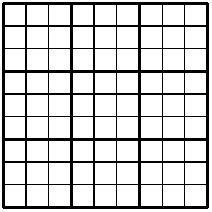
\includegraphics{sudoku}\\ \vspace{1cm}
\caption[Papan Permainan Sudoku]{Papan Permainan Sudoku} 
\end{figure}

\indent Pada beberapa kotak tersebut, ada orang yang menempati atau menulis angka 1-9; tujuan dari pemain adalah untuk mengisi setiap kotak tersebut dengan catatan bahwa tiap baris, tiap kolom dan tiap blok 3 x 3 berisi hanya satu kali saja angka 1-9.

\indent Pertanyaan yang sering ditanyakan adalah berapa banyaknya kemungkinan grid Sudoku. Artinya, berapa banyak cara yang dapat kita lakukan untuk mengisi kotak-kotak tersebut sesuai peraturan.

\indent Sudoku adalah kasus yang dikhususkan untuk kotak Latin yang merupakan n x n kotak yang masing-masing berisi angka 1 sampai n di setiap baris dan kolom. Perhitungan jumlah kotak Latin juga merupakan suatu masalah, karena tidak ada rumus umum yang dikenal. Ukuran yang telah berhasil adalah 11 x 11 kotak(9 x 9, 10 x 10, 11 x 11), dan metode yang digunakan adalah metode brute force. Jumlah langkah yang ditempuh untuk kotak Latin dengan ukuran 9 x 9 yang menggunakan brute force adalah $5524751496156892842531225600 \approx 5,525$ x $10^{27}$. Jumlah ini sangat besar, oleh karena itu, harus digunakan sedikit trik untuk menghitung dengan cara brute force untuk menyelesaikan sudoku dengan penggunaan waktu paling sedikit.

\section{Brute Force (Proof of Exhaustion)}
Proof of Exhaustion atau biasa dikenal metode brute force, adalah metode pembuktian matematis di mana pernyataan yang harus dibuktikan dibagi ke dalam kasus dengan jumlah terbatas atau kumpulan kasus setara dan masing-masing jenis kasus diperiksa untuk melihat apakah proposisi tersebut terbukti. Metode ini adalah metode yang membuktikan secara langsung. Sebuah pembuktian oleh proof of exhaustion berisi dua tahap:

\begin{enumerate}
	\item Sebuah bukti bahwa kasus lengkap; yaitu, bahwa setiap contoh dari pernyataan harus dibuktikan sesuai dengan kondisi (setidaknya) salah satu kasus.
	\item Sebuah bukti dari masing-masing kasus.
\end{enumerate}

\section{Block World Problem}
Block World adalah salah satu domain perencanaan yang paling terkenal dalam kecerdasan buatan(AI). Bayangkan satu set kubus (blok) diatas meja. Tujuannya adalah untuk membangun satu atau lebih tumpukan vertikal blok. Peraturannya adalah hanya satu blok dapat dipindahkan pada suatu waktu: baik dapat diletakkan di atas meja atau ditempatkan di atas blok lain. Karena itu, setiap blok pada waktu tertentu yang berada di bawah blok lain tidak dapat dipindahkan.

Kesederhanaan ini cocok untuk pendekatan AI, karena dunia dimodelkan sebagai satu set simbol abstrak yang dapat berhubungan satu sama lain.

\section{Ruang 3 Dimensi}
Ruang tiga dimensi adalah model tiga parameter geometris alam semesta fisika (tanpa mempertimbangkan waktu) dan semua materi yang dikenal ada. Ketiga dimensi dapat diberi label dengan tiga kombinasi dipilih dari panjang , lebar, tinggi, kedalaman, dan keluasan. Setiap tiga arah dapat dipilih, asalkan tidak semua terletak pada bidang yang sama.

Dalam fisika dan matematika, urutan angka n dapat dipahami sebagai lokasi dalam ruang n-dimensi. Ketika n = 3, himpunan semua lokasi tersebut disebut ruang tiga dimensi Euclidean. Hal ini umumnya diwakili oleh simbol $\Re^3$. Ruang ini hanya salah satu contoh dari berbagai ruang dalam tiga dimensi yang disebut 3-manifold.

\chapter{Penutup} %Penutup
\section{Kesimpulan}
\indent Banyak permainan tradisional yang telah dilupakan. Oleh karena itu, penulisan ilmiah ini dibuat. Permainan seperti Sudoku juga sudah berkurang peminatnya. Padahal, dulunya pernah populer di seluruh kalangan usia. Tulisan ini juga dibuat bertujuan untuk menarik perhatian pemain game zaman sekarang, mengingat semua game zaman sekarang dibuat dengan teknologi canggih.

\indent Sudoku bisa diselesaikan dengan banyak cara, salah satunya menggunakan brute force. Kotak sudoku berukuran 11 x 11 telah berhasil diselesaikan, termasuk juga 9 x 9 dan 10 x 10. Penyelesaian Sudoku dengan cara brute force tentu saja memakan waktu. Tetapi brute force yang digunakan tidak langsung dari awal, ada penyaringan tertentu sehingga menghemat waktu.

\indent Penyelesaian Sudoku cukup efektif, waktu yang digunakan juga relatif sedikit. Walapun waktu yang digunakan sedikit, jika ingin hasil \textit{instant} ketika dijalankan, masih memakan waktu cukup lama. Hardware yang digunakan juga harus memiliki spec yang tinggi. Hal ini disebabkan oleh pembuatan Sudoku berbasis 3D dan perhitungan yang cukup rumit.

\section{Saran}
Sangat direkomendasikan kepada pembaca yang ingin mempelajari lebih lanjut mengenai cara menyelesaikan sudoku dan membuat simulasi dalam ruang 3Dimensi karena 3Dimensi di zaman sekarang sudah dipakai pada kebanyakan permainan. Cara penyelesaian sudoku juga sangat penting untuk mempelajari
metode-metode yang bisa digunakan.

\begin{thebibliography}{9}

%@article{felgenhauer2006mathematics,
  %title={Mathematics of sudoku I},
  %author={Felgenhauer, Bertram and Jarvis, Frazer},
  %journal={Mathematical Spectrum},
  %volume={39},
  %number={1},
  %pages={15--22},
  %year={2006},
  %publisher={[Oxford, Eng.] Oxford University Press.}
%}
\bibitem{}
	Felgenhauer, Bertram and Jarvis, Frazer.
	\emph{Mathematics of sudoku I}.
	[Oxford, Eng.] Oxford University Press,
	2006.

%@inproceedings{gupta1991complexity,
  %title={Complexity Results for Blocks-World Planning.},
  %author={Gupta, Naresh and Nau, Dana S and others},
  %booktitle={AAAI},
  %volume={91},
  %pages={629--633},
  %year={1991},
  %organization={Citeseer}
%}
\bibitem{}
	Gupta, Naresh and Nau, Dana S and others.
	\emph{Complexity Results for Blocks-World Planning}.
	1991.

%@article{chenowet1991np,
  %title={On the NP-hardness of blocks world},
  %author={Chenowet, Stephen V},
  %year={1991}
%}
\bibitem{}
	Chenowet, Stephen V.
	\emph{On the NP-hardness of blocks world}.
	1991.
	
%Reid, D. A; Knipping, C (2010), Proof in Mathematics Education: Research, Learning, and Teaching, Sense Publishers, p. 133, ISBN 978-9460912443.

\bibitem{}
	Reid, D. A.
	\emph{Proof in Mathematics Education: Research, Learning, and Teaching}.
	Sense Publishers.
	2010.

\end{thebibliography}
\end{document}
 